\section{Bias injection test}

\label{sec:bias_injection}
To understand the effect of a bias which effects only very high 
\mht bins on the validation procedure a bias injection test is carried out.
The prediction in the final bin only is varied and the effect on the 
overall pull studied. The results are shown for the symmetric jet categories only
as for asymmetric categories the final \mht bin dominates the fit. This is 
an extreme test of the ability to probe bias using the linear fit. 
Fig.~\ref{fig:biasInjTest} displays the results of this test showing
the pull distribution is sensitive to such a bias. In Fig.~\ref{fig:biasSyst} the 
change in predicted systematic is shown for the case of halving the prediction in the last bin. 
This shows an overall substantial increase in the systematics predicted.

\begin{figure}[h!]
  \centering
  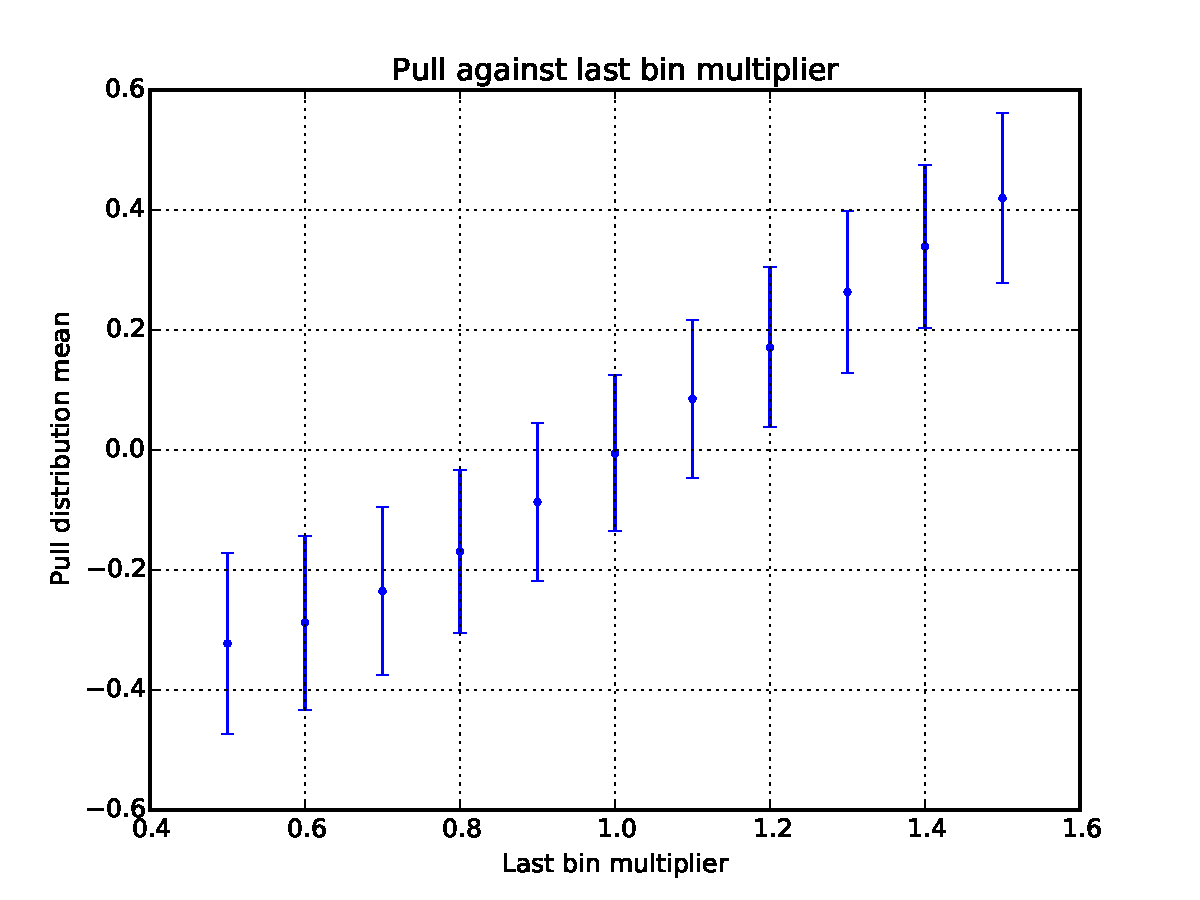
\includegraphics[width=0.5\textwidth]{figures/template/biasInjTest.pdf}
  \caption{\label{fig:biasInjTest} Mean pull against last bin multiplier for 
  the \mj control region showing the linear polynomial is sensitive to a bias effecting the final bin only.}
\end{figure}
\begin{figure}[h!]
  \centering
  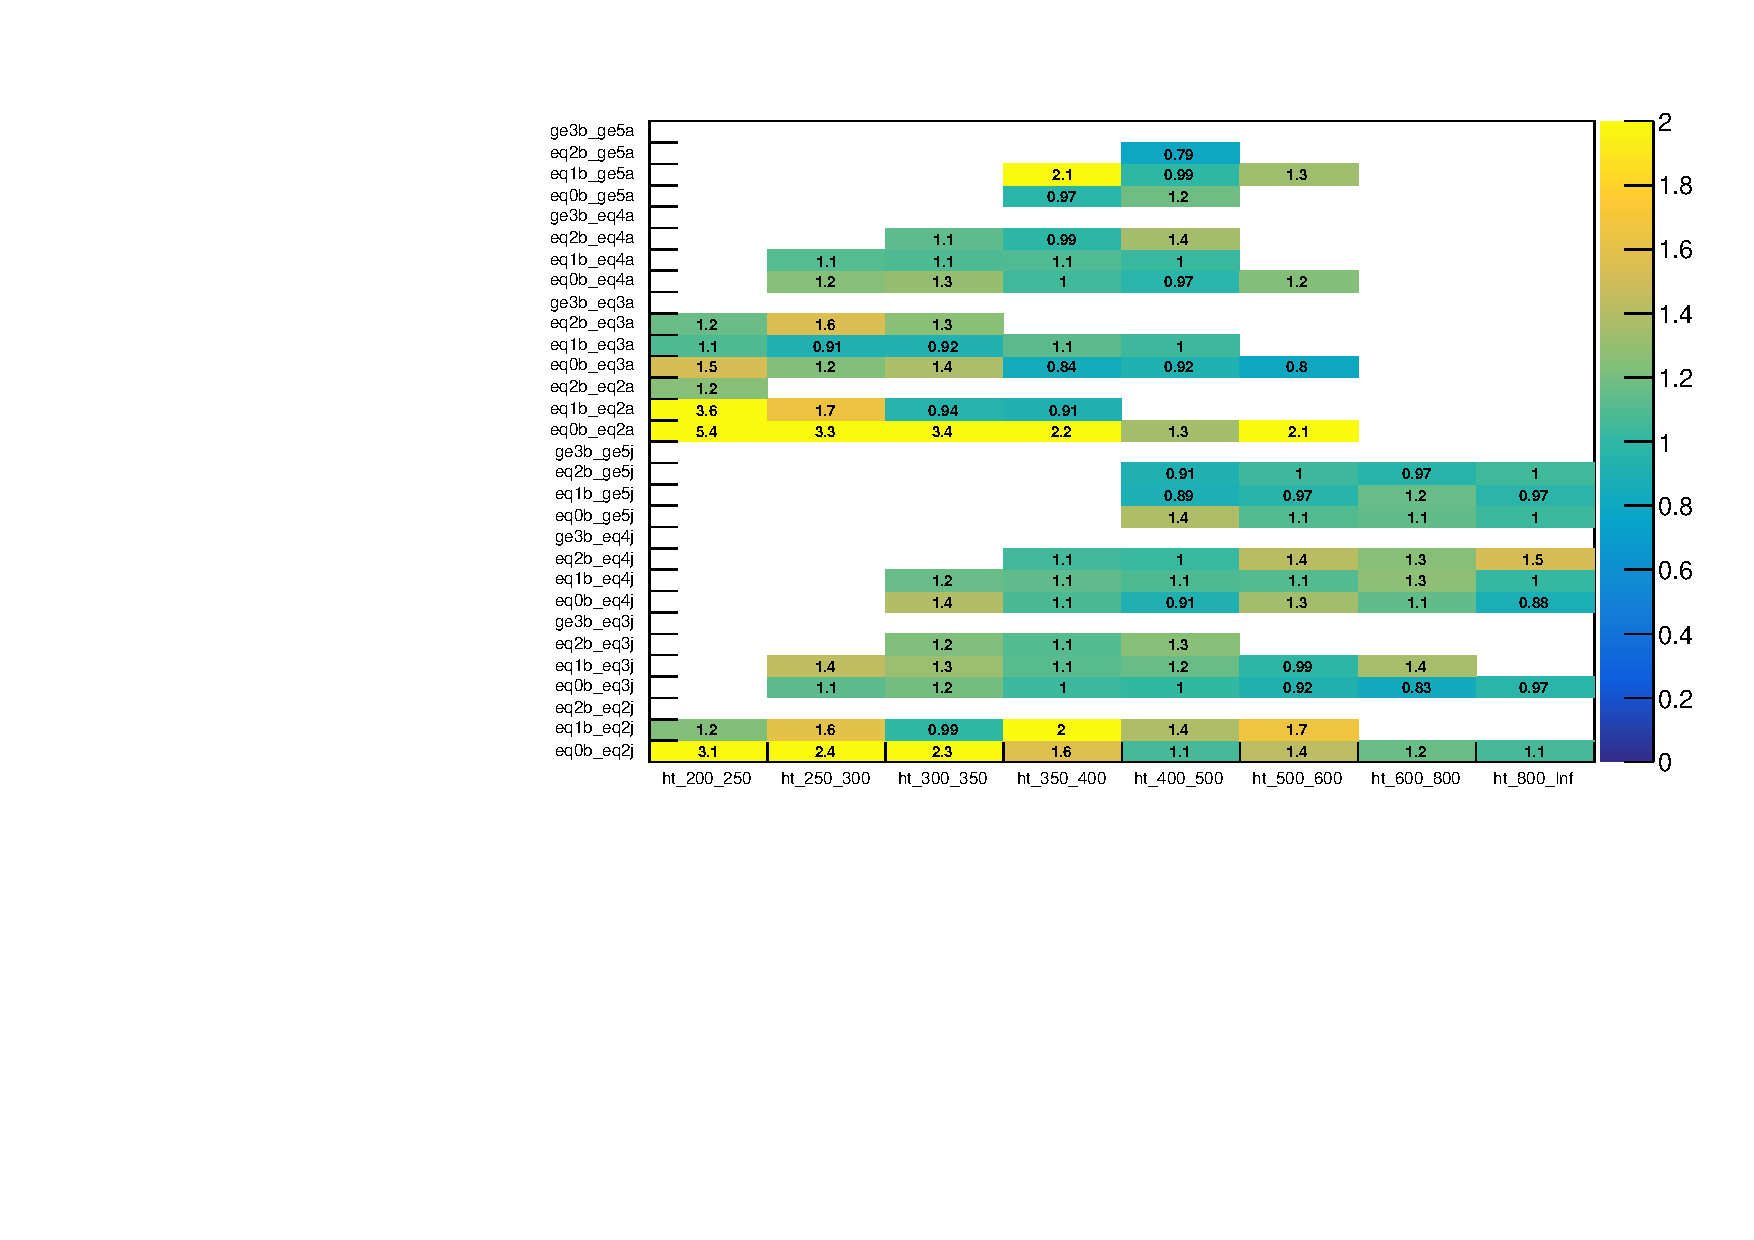
\includegraphics[width=0.5\textwidth]{figures/template/biasSystTest.pdf}
  \caption{\label{fig:biasSyst} Change in systematic parameter when the prediction in the last bin
  is halved}
\end{figure}
